\documentclass{journal}
\usepackage{graphicx}
\usepackage{siunitx}


\begin{document}
\title{AP Calculus Final Project}
\author{Joshua Morin-Baxter, Alan Zhu, Nathan Wiley, and George Hong}
\date{\today}

\maketitle

\begin{abstract}
This is an analysis of data taken from the GOSH Flight Path Predictor\textsuperscript{TM}.
Four separate sets of data were analyzed:
temperature vs. density, wind velocity vs. pressure, wind angle vs. wind velocity, and wind velocity vs. altitude.
Each is discussed in more depth in subsequent parts.
\end{abstract}

\part{Wind Velocity vs. Altitude}
This data seems to have two points that are of great interest.
\begin{figure}[h]
\centering
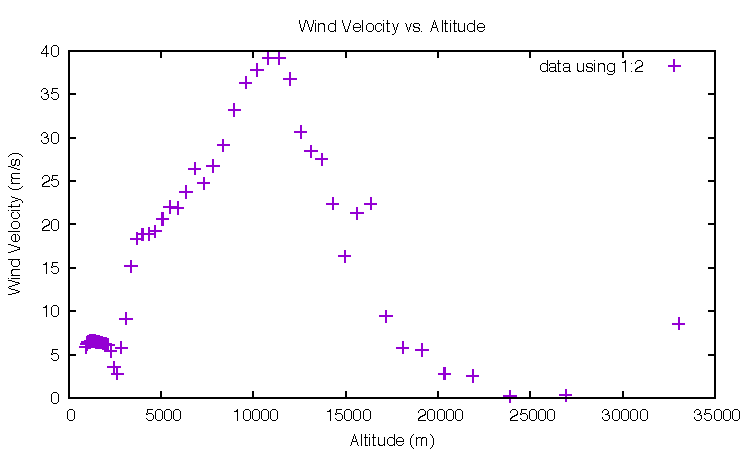
\includegraphics{josh-images/figure1.pdf}
\caption{Test}

\end{figure}


\part{Temperature Vs. Density}

\part{Wind Velocity vs. Pressure}

\part{Wind Angle vs. Wind Velocity}



\end{document}
